\newpage
\section{Test 2}
\label{Sec:test_2}

In the second test setting rover stands still on the horizontal plane during first 50 seconds of the simulation.
However, after 50 seconds from the beginning of the simulation a constant torque $\tau = 2N$ is applied in one of the steering axes (steering axis FL)
causing its rotational motion with linear velocity. Wheel makes two full rotations around its vertical steering axis (FL). 
Other external forces acting on the rover are the gravity and ground reaction. Initial position of the center of mass of the robot
has been set to (x, y, z) = (10, 0.55, 10). 

\begin{figure}[H]
  \centering
    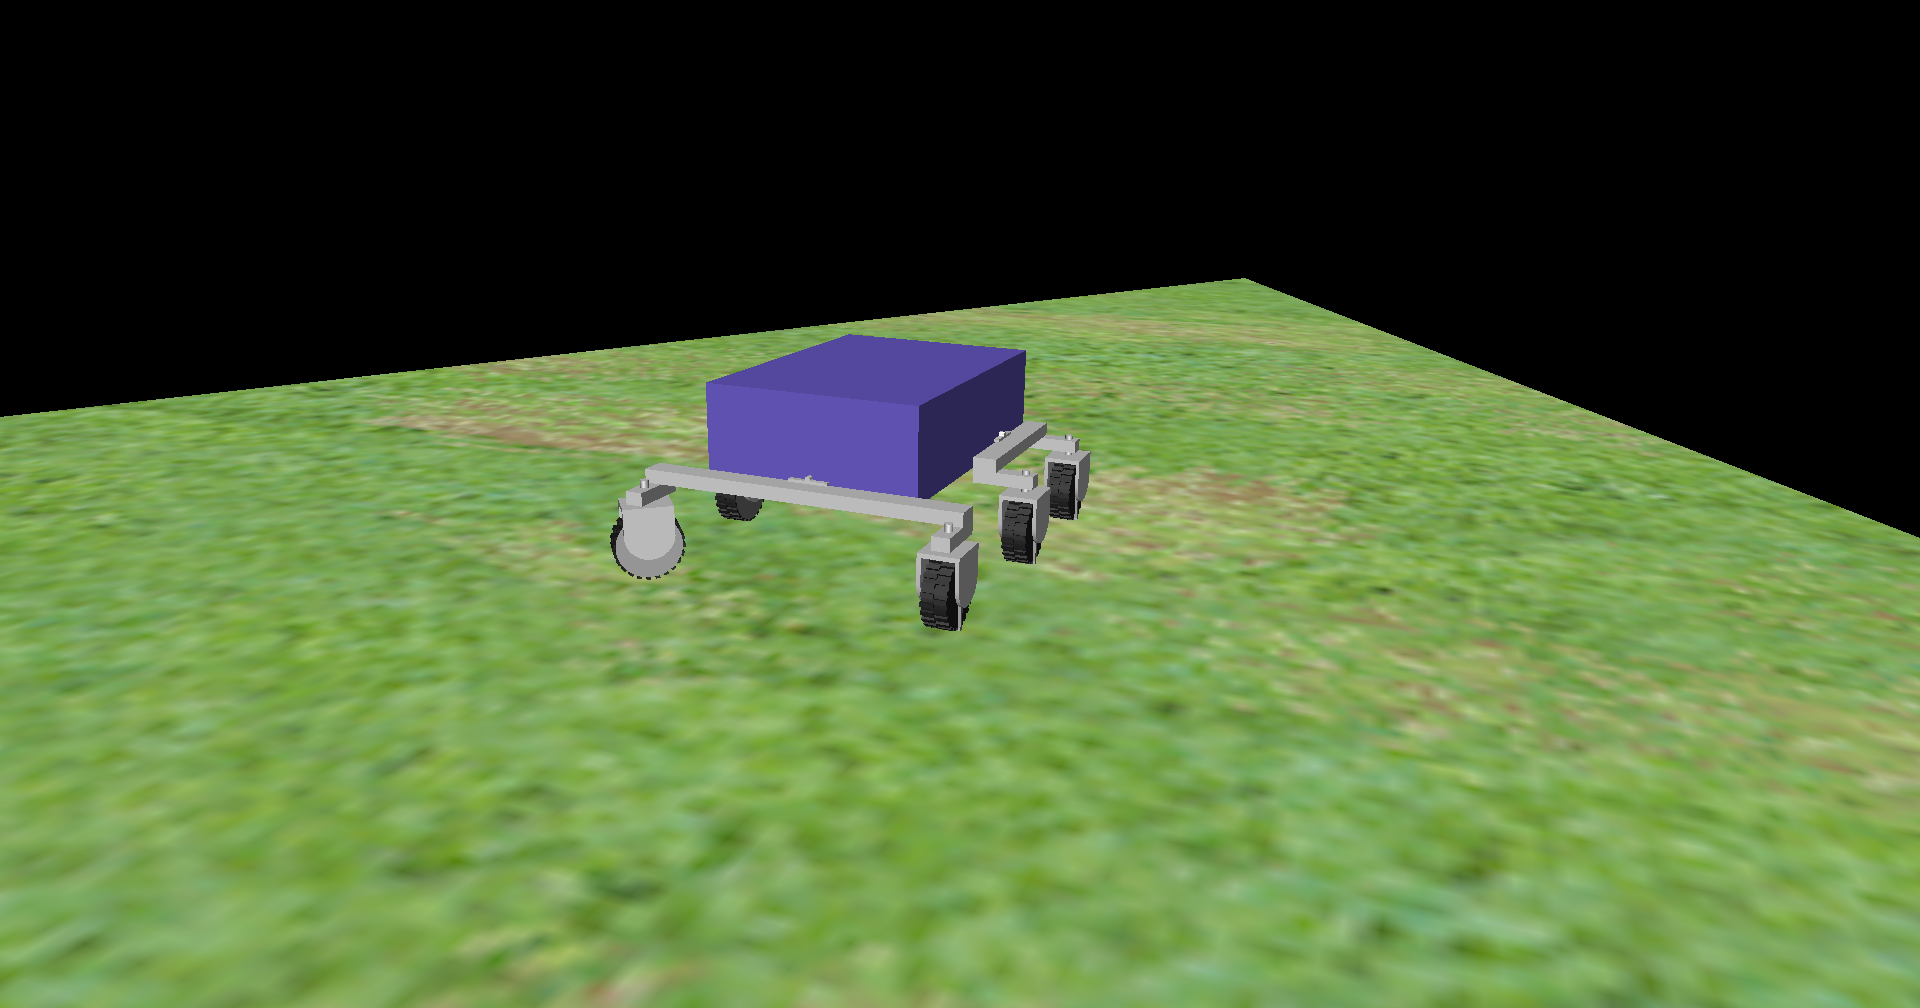
\includegraphics[width=0.8\textwidth]{run_2}
  \caption{Second test scenario}
\end{figure}

\noindent In this case, following quantities have been plotted:

\begin{itemize}
  \item $v_{FL}$ - angular velocity of the FL axis
\end{itemize}

\begin{figure}[H]
  \centering
    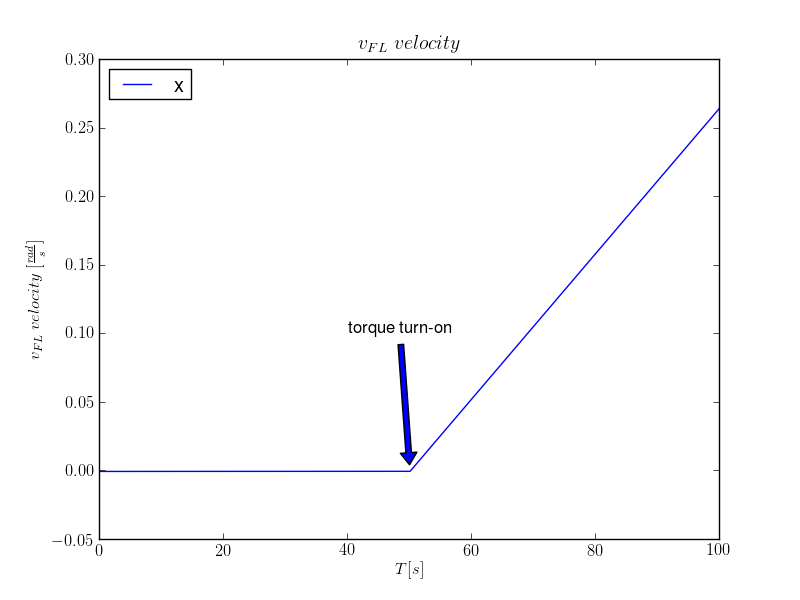
\includegraphics[width=0.8\textwidth]{vFL}
  \caption{$v_{FL}$}
\end{figure}

\begin{itemize}
  \item $x_{FL}$ - $q$ coordinate corresponding to the FL axis
\end{itemize}

\begin{figure}[H]
  \centering
    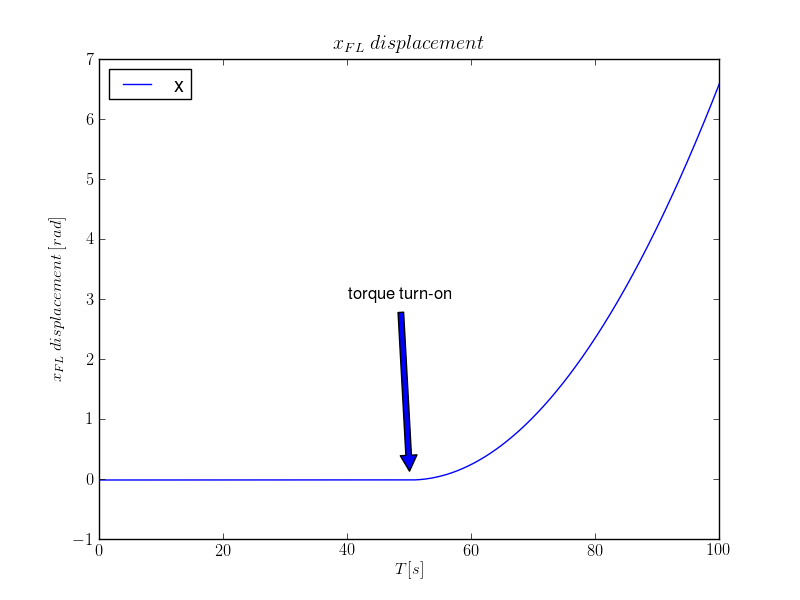
\includegraphics[width=0.8\textwidth]{xFL}
  \caption{$x_{FL}$}
\end{figure}

\begin{itemize}
  \item $\lambda_{N}$ - normal component of the contact force (impulsion) for each wheel
\end{itemize}

\begin{figure}[H]
  \centering
    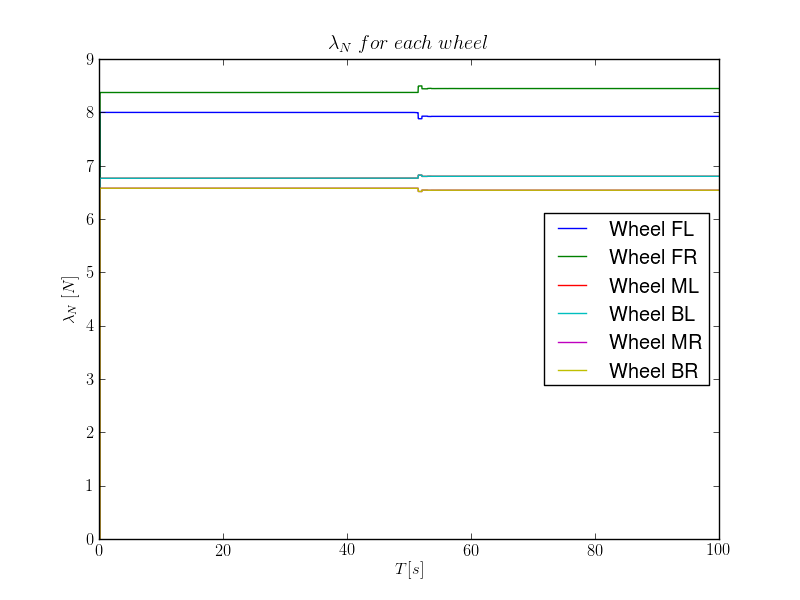
\includegraphics[width=0.8\textwidth]{lambdaN2}
  \caption{$\lambda_{N}$}
\end{figure}

\begin{figure}[H]
  \centering
    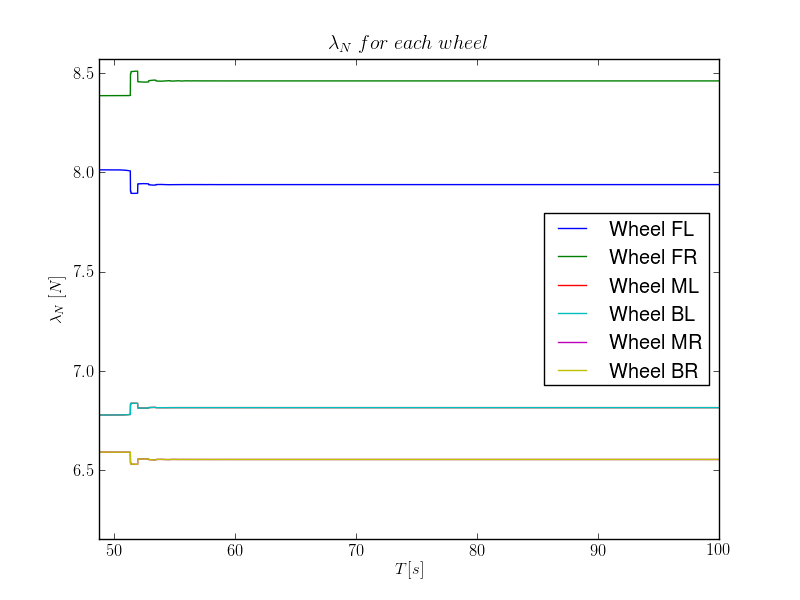
\includegraphics[width=0.8\textwidth]{lambdaN2steady}
  \caption{$\lambda_{N}$ zoom view}
\end{figure}

\begin{itemize}
  \item $\lambda_{T_x}$ - tangential component of the contact force in the x direction for each wheel
\end{itemize}

\begin{figure}[H]
  \centering
    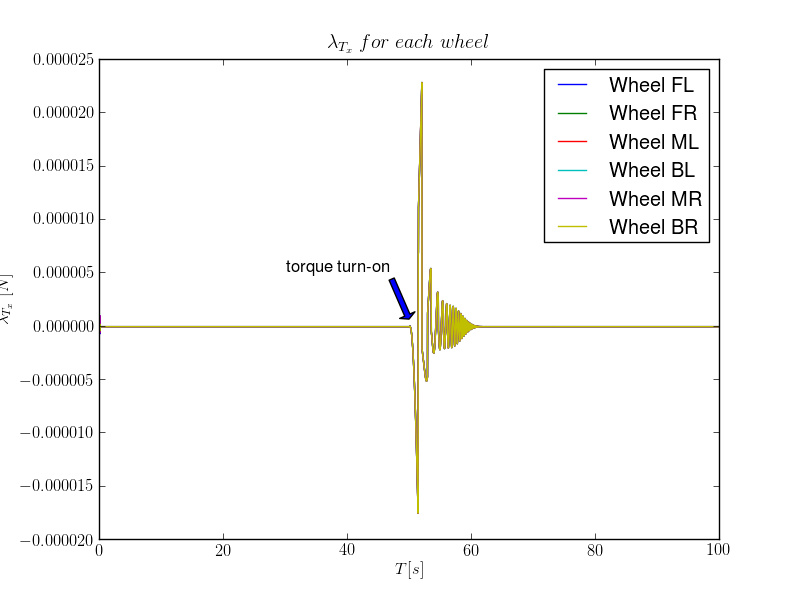
\includegraphics[width=0.8\textwidth]{lambdaTx2}
  \caption{$\lambda_{T_x}$}
\end{figure}

\begin{itemize}
  \item $\lambda_{T_z}$ - tangential component of the contact force in the z direction for each wheel
\end{itemize}

\begin{figure}[H]
  \centering
    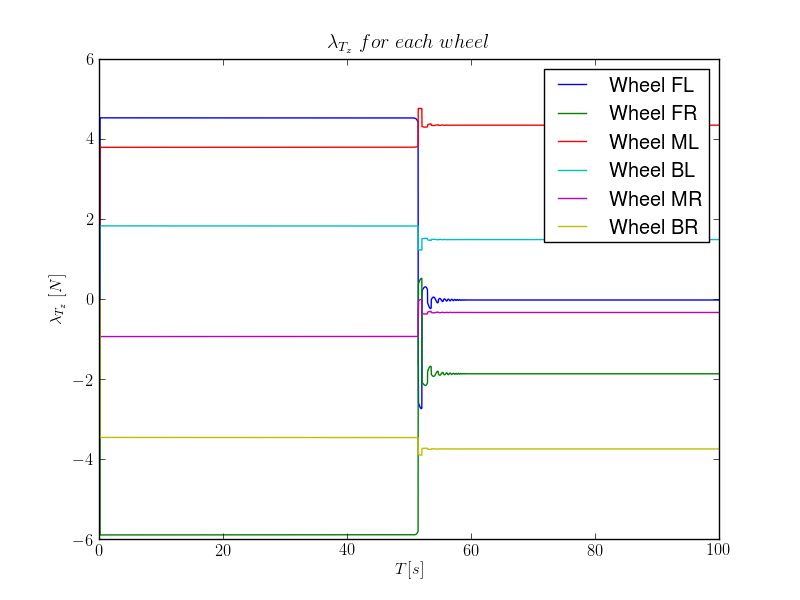
\includegraphics[width=0.8\textwidth]{lambdaTz2}
  \caption{$\lambda_{T_z}$}
\end{figure}

\begin{itemize}
  \item $y_{N}$ - gap function (distance between contact point and the constraint function) for each wheel
\end{itemize}

\begin{figure}[H]
  \centering
    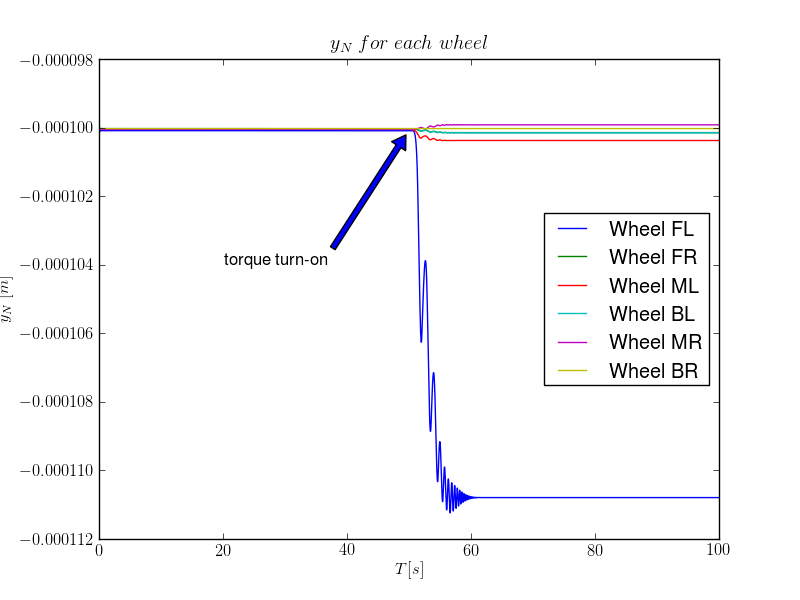
\includegraphics[width=0.8\textwidth]{yN2}
  \caption{$y_{N}$}
\end{figure}

\begin{itemize}
  \item $\dot{y}_{N}$ - normal component of the local contact velocity for each wheel
\end{itemize}

\begin{figure}[H]
  \centering
    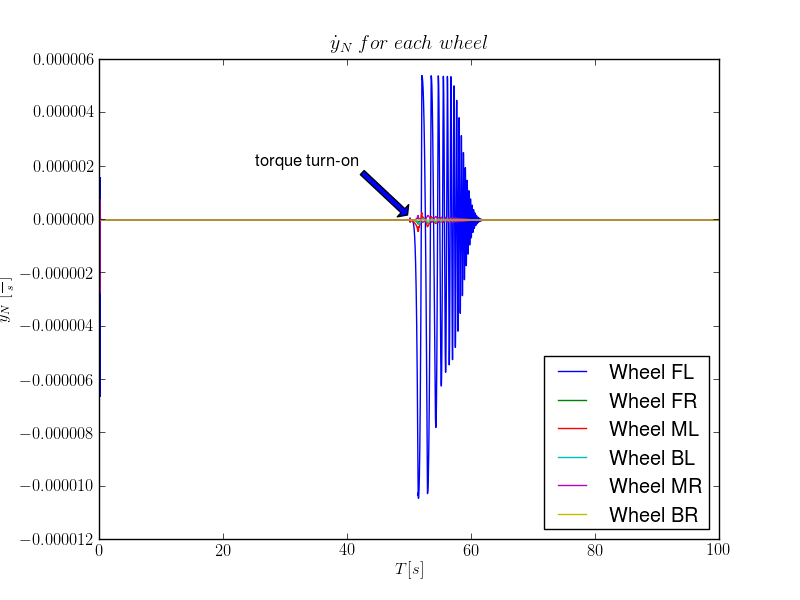
\includegraphics[width=0.8\textwidth]{yNdot2}
  \caption{$\dot{y}_{N}$}
\end{figure}

\begin{itemize}
  \item $\dot{y}_{T_x}$ - tangential component x of the local contact velocity for each wheel
\end{itemize}

\begin{figure}[H]
  \centering
    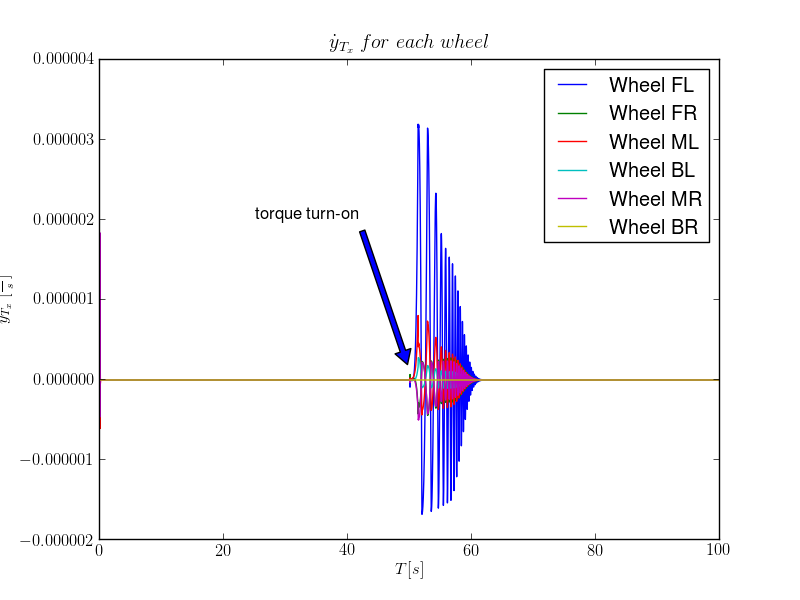
\includegraphics[width=0.8\textwidth]{yTxdots2}
  \caption{$\dot{y}_{T_x}$}
\end{figure}

\begin{itemize}
  \item $\dot{y}_{T_z}$ - tangential component z of the local contact velocity for each wheel
\end{itemize}

\begin{figure}[H]
  \centering
    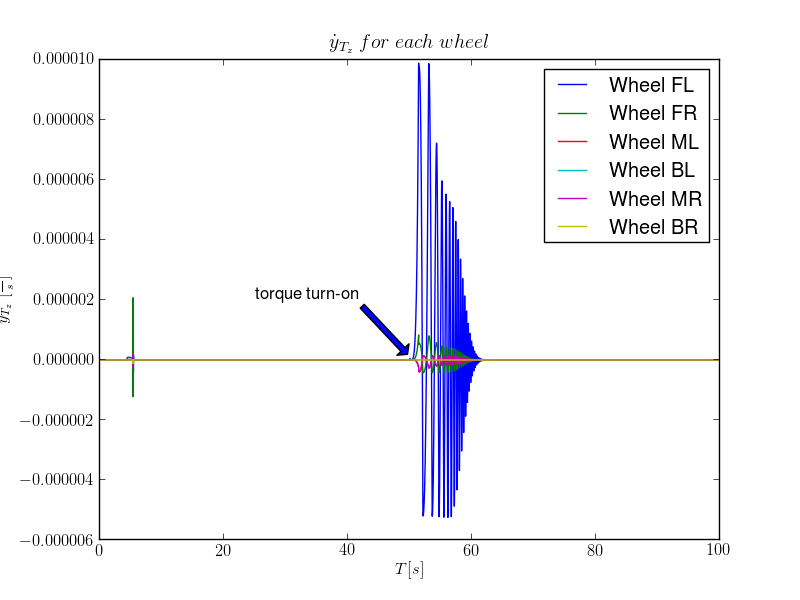
\includegraphics[width=0.8\textwidth]{yTzdots2}
  \caption{$\dot{y}_{T_z}$}
\end{figure}
